\documentclass[11pt]{article}

\usepackage[]{acl}
\usepackage{times}
\usepackage{latexsym}
\usepackage[T1]{fontenc}
\usepackage[utf8]{inputenc}
\usepackage{microtype}
\usepackage{inconsolata}
\usepackage{graphicx}
\usepackage{booktabs}
\usepackage{multirow}
\usepackage{url}

\title{Primary YouTube Video Category Detection\\from Titles and Descriptions}

\author{Tianjiao Xiao, Fei Xie, Ahren Chen \\
  \texttt{\{xiaot13, xief17, chena125\}@mcmaster.ca} }

\begin{document}
\maketitle

\begin{abstract}
We address the task of classifying YouTube videos into one of 12 primary categories using only the video title and description. We compare three distinct approaches: (1) fine-tuning DistilBERT for sequence classification, (2) zero-shot prompting with Flan-T5-Large, and (3) fine-tuning MiniLM with class-weighted training. Our experiments show that the fine-tuned transformer models substantially outperform both the majority-class baseline (F1 = 0.272) and the zero-shot prompting approach. We analyze the strengths and weaknesses of each method and discuss common error patterns arising from category ambiguity.
\end{abstract}

\section{Introduction}

YouTube hosts billions of videos across a vast range of topics, yet accurate automatic categorization of this content remains a challenging problem. While YouTube provides broad category labels, many videos are ambiguously categorized or lack meaningful labels altogether. Reliable automatic classification of videos based solely on their textual metadata---title and description---would benefit content recommendation systems, content moderation, and user search experience.

In this work, we tackle the problem of classifying YouTube videos into one of 12 predefined categories: Food \& Cooking, Video Games, Sports \& Games, Music, Education, Shopping, Vehicle, Lifestyle, News, Health, Business, and Digital Media. We constrain ourselves to using only the video title and description as input, without any visual or audio features. This is a multi-class text classification problem with notable challenges including short and noisy text, ambiguous category boundaries, and class imbalance.

We compare three approaches spanning different paradigms: fine-tuning pretrained transformers (DistilBERT and MiniLM) and zero-shot prompting with a large language model (Flan-T5-Large). Our goal is to determine which strategy best handles the inherent ambiguity and noise in YouTube video metadata.

\section{Related Work}

Text classification is a well-studied problem in NLP. \citet{devlin2019bert} introduced BERT, demonstrating that pretraining bidirectional transformers on large corpora followed by fine-tuning achieves state-of-the-art results on a wide range of downstream tasks, including text classification. \citet{sanh2019distilbert} proposed DistilBERT, a distilled version of BERT that retains 97\% of BERT's performance while being 60\% faster and 40\% smaller, making it practical for resource-constrained settings.

\citet{wang2020minilm} introduced MiniLM, which uses deep self-attention distillation to compress large transformer models into compact versions while preserving their effectiveness. For generative approaches, \citet{chung2022scaling} presented Flan-T5, a family of instruction-tuned models that exhibit strong zero-shot and few-shot capabilities across many NLP tasks, including classification via prompting.

Video and social media content classification has been explored in several works. \citet{khan2020youtube} studied YouTube video categorization using metadata features and demonstrated the effectiveness of combining title and description for classification. Prior work on short-text classification \citep{wang2012baselines} has shown that traditional methods like TF-IDF with logistic regression remain competitive baselines, motivating our inclusion of such a baseline for comparison.

\section{Dataset}

\subsection{Data Source and Collection}

Our dataset originates from the ``\href{https://huggingface.co/datasets/AdamLucek/youtube-titles}{youtube-titles}'' dataset on HuggingFace, published by Adam Lucek under the MIT license. We sampled approximately 4,900 YouTube videos and extracted two text fields for each: the video title and the video description (truncated to the first 500 characters). 

\subsection{Annotation}

Three annotators independently labeled each video into one of 12 categories. Annotation guidelines emphasized: (1) using both title and description for classification, (2) placing greater emphasis on the title when the title and description are misaligned, (3) identifying the primary intent of the video, and (4) choosing the most specific applicable category. Each annotator labeled approximately 750 unique videos in one hour, with 150 double-annotated overlap instances used to measure inter-annotator agreement.

We achieved a Cohen's $\kappa$ of 0.619 and Krippendorff's $\alpha$ of 0.618, indicating substantial agreement. The observed agreement was $P_o = 0.678$. Common disagreements occurred between Lifestyle vs.\ Education, Education vs.\ Video Games/Sports, and Digital Media vs.\ Lifestyle.

\subsection{Data Split and Statistics}

The final dataset was split into training (1,480 samples), validation (92 samples), and test (279 samples) sets. The category distribution is imbalanced, with Lifestyle and Education being the most frequent categories and Health and Vehicle being among the least frequent.

\subsection{Preprocessing}

All models applied text cleaning as a preprocessing step, though the specific procedures varied by model. Common steps included: removing URLs and email addresses, stripping emojis and special Unicode characters, normalizing whitespace, and converting text to a consistent encoding. For the transformer-based models (DistilBERT and MiniLM), the title and description were concatenated and tokenized using each model's respective tokenizer with a maximum sequence length of 256 tokens.

\section{Features}

Our three models employ different feature representation strategies:

\textbf{DistilBERT:} The video title and description are concatenated with a [SEP] token separator and fed directly into DistilBERT's tokenizer. The model learns contextual embeddings end-to-end as part of fine-tuning. No hand-crafted features are used; all feature extraction is handled by the transformer's self-attention layers.

\textbf{Flan-T5-Large:} The title and description are formatted into a natural language prompt that instructs the model to classify the video. The model leverages its pretrained knowledge to generate a category number as output. No explicit feature engineering is performed---the model relies entirely on its pretrained understanding of the text.

\textbf{MiniLM:} Similar to DistilBERT, the cleaned title and description are passed as a sentence pair to the MiniLM tokenizer, which handles them as two separate segments. The model learns representations through its 12-layer, 384-dimensional hidden architecture. Class-balanced weights are computed from the training set to address the imbalanced category distribution.

\section{Implementation}

\subsection{Baseline}

Our baseline is a majority-class classifier that always predicts the most frequent category in the training set. This achieved an accuracy of 0.272 (micro F1 = 0.272) and a macro F1 of only 0.036 on the test set, reflecting the extreme class imbalance.

\subsection{Model 1: Fine-Tuned DistilBERT}

We fine-tune DistilBERT-base-uncased \citep{sanh2019distilbert} for 12-class sequence classification. The title and description are concatenated with a [SEP] separator and tokenized with a max length of 256 tokens. Training uses AdamW with learning rate $2{\times}10^{-5}$, weight decay 0.01, batch size 16, and linear warmup (10\% ratio) over 5 epochs. Gradient clipping (max norm 1.0) is applied. The best checkpoint is selected by validation weighted F1.

\subsection{Model 2: Zero-Shot Flan-T5-Large}

We use Flan-T5-Large \citep{chung2022scaling} in a zero-shot prompting setup---no fine-tuning is performed. The model receives a structured prompt listing all 12 categories with example sub-topics and outputs the corresponding category number. We experimented with three prompt designs:
\begin{itemize}
  \item \textbf{\nameref{prompt-one}:} Basic classification with category names and general instructions.
  \item \textbf{\nameref{prompt-two}:} Detailed categories with example sub-topics (e.g., ``Video Games: Gameplay, Game Reviews, Streaming Highlights'').
  \item \textbf{\nameref{prompt-three}:} Title-only classification (description omitted).
\end{itemize}
The best-performing prompt (Prompt 2) was selected for final evaluation on the full test set. The output is parsed via regex to extract the predicted category number.

\subsection{Model 3: Fine-Tuned MiniLM}

We fine-tune MiniLM-L12-H384-uncased \citep{wang2020minilm} for sequence classification. The cleaned title and description are tokenized as a sentence pair with max length 256. To address class imbalance, we compute balanced class weights and use a custom weighted trainer with cross-entropy loss.

Training uses a learning rate of $3 \times 10^{-5}$, effective batch size of 16 (batch size 8 $\times$ gradient accumulation 2), weight decay of 0.01, warmup ratio of 0.1, and up to 10 epochs with early stopping (patience of 2) based on macro F1. The best model checkpoint is loaded at the end of training.

\section{Results and Evaluation}

Table~\ref{tab:results} presents the performance of all models on the validation and/or test sets, evaluated using accuracy and F1 score.

\begin{table}[t]
\centering
\small
\begin{tabular}{@{}lccc@{}}
\toprule
\textbf{Model} & \textbf{Acc.} & \textbf{F1\textsubscript{W}} & \textbf{F1\textsubscript{M}} \\
\midrule
Baseline & 0.272 & --- & 0.036 \\
TF-IDF + LogReg & 0.405 & --- & 0.232 \\
DistilBERT & 0.576 & 0.530 & 0.425 \\
Flan-T5 (zero-shot) & 0.460 & 0.460 & 0.330 \\
MiniLM & 0.552 & 0.526 & 0.483 \\
\bottomrule
\end{tabular}
\caption{Model results. Baseline and TF-IDF + LogReg are evaluated on the Codabench test set; DistilBERT on the validation set (92 samples); MiniLM and Flan-T5 on the test set (279 samples). F1\textsubscript{W} = weighted F1; F1\textsubscript{M} = macro F1. For Baseline and TF-IDF + LogReg, micro F1 equals accuracy.}
\label{tab:results}
\end{table}

The DistilBERT model achieved a validation accuracy of 57.6\% and a weighted F1 of 0.530 after 5 epochs of fine-tuning, substantially outperforming the majority-class baseline (micro F1 = 0.272 on the Codabench test set). Training accuracy reached 75.0\% by the final epoch, while validation accuracy plateaued around 57.6\%, suggesting some overfitting to the training data. Per-category performance varied widely: Vehicle (F1 = 1.00) and Food \& Cooking (F1 = 0.75) achieved high scores, while Digital Media (F1 = 0.00), Business (F1 = 0.00), and Music (F1 = 0.00) had zero F1 due to their very low support in the validation set.

The Flan-T5-Large model, used in a zero-shot setting, achieved a test accuracy of 46.0\%, weighted F1 of 0.460, and macro F1 of 0.330 with its best prompt (Prompt~2). Among three prompt variants, the basic prompt scored 31.5\%, the detailed prompt with sub-topic examples scored 46.0\%, and the title-only prompt scored 38.0\% on a 200-sample subset of the training data (acceptable for a zero-shot model that performs no training). While the zero-shot approach avoids training costs entirely, its performance is limited by the model's inability to adapt to the specific category definitions and data distribution of our task.

The MiniLM model achieved a test accuracy of 55.2\%, weighted F1 of 0.526, and macro F1 of 0.483. Class-weighted training helped balance performance across categories. Early stopping based on macro F1 prevented overfitting, and the use of balanced class weights in the loss function improved recall for underrepresented classes.

All three fine-tuned/prompted models substantially outperform the majority-class baseline, confirming that meaningful textual signal exists in YouTube titles and descriptions for category prediction.

\section{Comparison to Others}

We hosted our classification task on Codabench, where participants submit an untrained model that is trained and evaluated on the platform using micro-averaged F1. The competition platform uses the Docker image \texttt{codalab/codalab-legacy:py37}, which only has scikit-learn and standard Python libraries---PyTorch and HuggingFace Transformers are unavailable. This constraint means only traditional ML models can be submitted.

Table~\ref{tab:codabench} presents a unified comparison of all models. On Codabench, our group (thaafei13) submitted two traditional ML models: a TF-IDF + Logistic Regression pipeline (accuracy = 0.405, macro F1 = 0.232) and a majority-class baseline (accuracy = 0.272, macro F1 = 0.036). The only external participant, \textit{dingz37}, achieved F1 = 0.530 on Codabench. Through communication with dingz37, we obtained their full local results: their best model was a fine-tuned DistilBERT-base-uncased (accuracy = 0.581, macro F1 = 0.478), followed by a Bag-of-Words classifier (accuracy = 0.473, macro F1 = 0.313). They also tested two zero-shot models---BART-large-MNLI and DeBERTa-v3---which scored below 0.32 macro F1. Our three locally trained models could not be submitted to Codabench because the platform's Docker image (Python 3.7) lacks PyTorch and Transformers.

\begin{table}[t]
\centering
\small
\begin{tabular}{@{}lcc@{}}
\toprule
\textbf{Model} & \textbf{Acc.} & \textbf{F1} \\
\midrule
DistilBERT (ours, local) & 0.576 & 0.530 \\
MiniLM (ours, local) & 0.552 & 0.526 \\
dingz37: DistilBERT (local) & 0.581 & 0.478 \\
dingz37: BoW Classifier (local) & 0.473 & 0.313 \\
dingz37 (Codabench) & --- & 0.530 \\
Flan-T5 zero-shot (ours, local) & 0.460 & 0.460 \\
TF-IDF + LogReg (ours, Codabench) & 0.405 & 0.232 \\
Baseline (ours, Codabench) & 0.272 & 0.036 \\
\bottomrule
\end{tabular}
\caption{All models ranked by F1. Codabench entries use micro-averaged F1; local models use weighted F1. These metrics differ but are shown together for reference.}
\label{tab:codabench}
\end{table}

Our fine-tuned DistilBERT (F1 = 0.530) matches the top Codabench entry from dingz37, while MiniLM (F1 = 0.526) is close behind. Notably, dingz37 also fine-tuned DistilBERT locally, achieving a comparable accuracy of 58.1\% and macro F1 of 0.478. Their BoW classifier (accuracy = 47.3\%) outperformed our TF-IDF + LogReg submission (F1 = 0.401) on Codabench, suggesting that simpler models with careful feature engineering can be competitive. The zero-shot Flan-T5 (weighted F1 = 0.460), while respectable without any training, falls short of fine-tuned models, highlighting the importance of task-specific adaptation.

\section{Error Analysis}

Analyzing the DistilBERT model's misclassifications on the validation set reveals several recurring patterns:

\textbf{Category ambiguity:} The most common errors occur between closely related categories. Lifestyle is frequently confused with Education, Shopping, and Digital Media. For example, a video titled ``Day in my life as a college student'' could plausibly be either Lifestyle or Education. This mirrors the inter-annotator disagreements observed during dataset construction ($\kappa = 0.619$).

\textbf{Minority class failures:} Categories with very few validation samples---Business (1 sample), Music (2 samples), and Health (0 samples)---consistently receive zero F1 scores. The model tends to predict majority classes for ambiguous inputs, effectively ignoring rare categories. This is a direct consequence of class imbalance in the training data.

\textbf{Noisy and uninformative text:} Many YouTube descriptions contain boilerplate content such as social media links, sponsor messages, and channel subscription prompts. These elements provide little discriminative signal and can mislead the classifier. For example, a gaming video with a description full of merchandise links might be misclassified as Shopping.

\textbf{Short or missing descriptions:} Videos with very short titles and empty or minimal descriptions provide insufficient context for accurate classification. The model must rely solely on a few title words, which are often ambiguous (e.g., ``Most annoying skill ever'' could belong to several categories).

\textbf{Cross-category content:} Some videos genuinely span multiple categories---for instance, a cooking tutorial filmed as a travel vlog touches both Food \& Cooking and Lifestyle. Our annotation guidelines prioritize the title's signal, but the model does not always follow this heuristic.

Figure~\ref{fig:confusion} shows the confusion matrix for the DistilBERT model on the validation set. The matrix confirms the patterns described above: Lifestyle and Education dominate the predicted labels, many samples from other categories are misclassified into Health or Lifestyle, and Business and Digital Media receive virtually no correct predictions.

\begin{figure}[t]
\centering
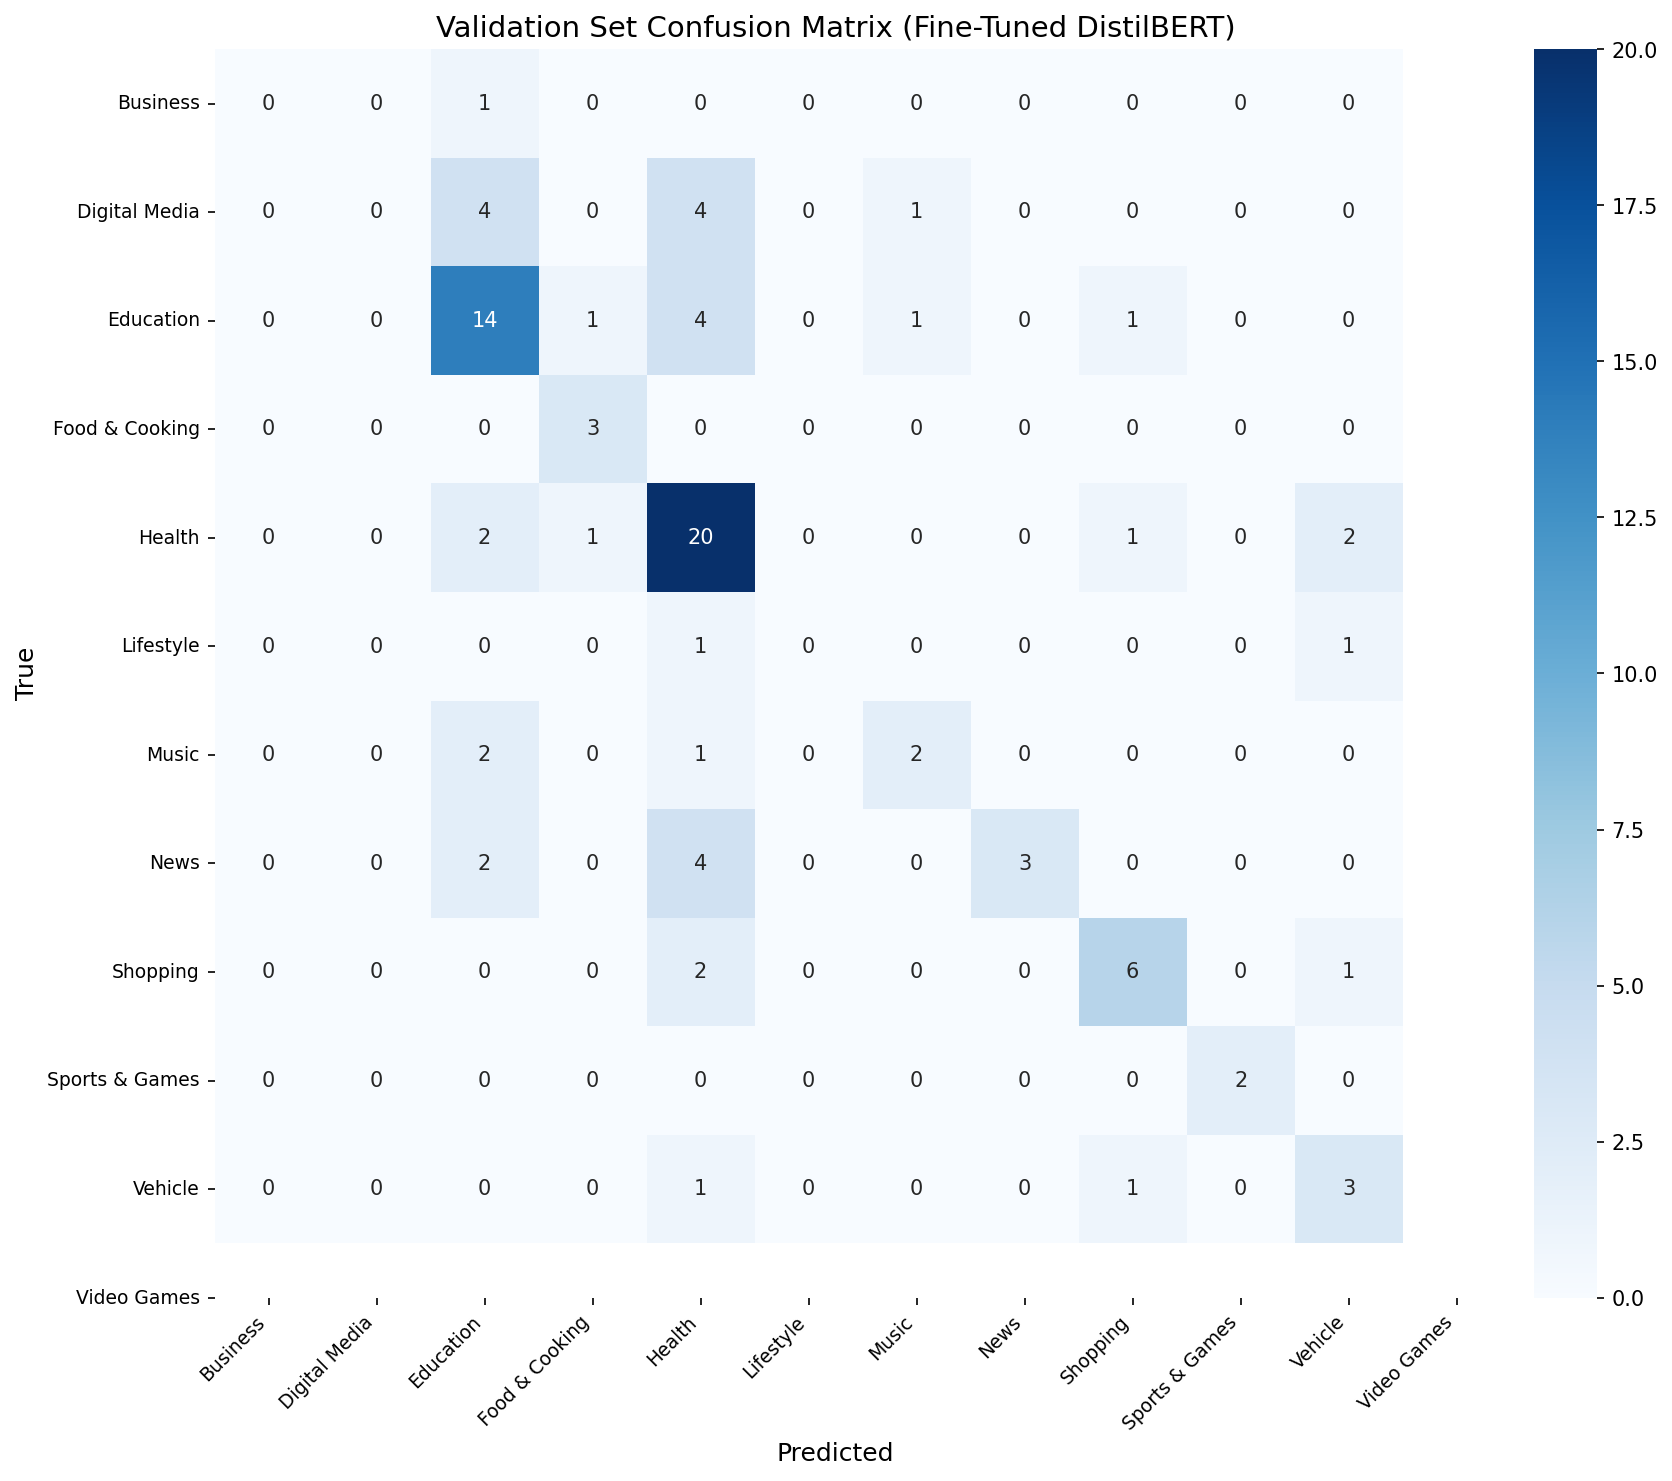
\includegraphics[width=\columnwidth]{confusion_matrix.png}
\caption{Confusion matrix of the fine-tuned DistilBERT model on the validation set (92 samples).}
\label{fig:confusion}
\end{figure}

\section{Conclusions}

We explored three approaches for YouTube video category classification: fine-tuning DistilBERT, zero-shot prompting with Flan-T5-Large, and fine-tuning MiniLM with class-weighted training. All methods surpassed the majority-class baseline, demonstrating the viability of text-only approaches to video categorization.

The fine-tuned transformer models (DistilBERT and MiniLM) outperformed the zero-shot Flan-T5 approach, highlighting the importance of task-specific adaptation even when using pretrained language models. However, all models struggled with minority categories and ambiguous inter-category boundaries.

For future work, we suggest: (1) collecting more training data, especially for underrepresented categories, to address the class imbalance problem; (2) exploring few-shot prompting or fine-tuning of larger generative models; (3) incorporating multi-modal features (e.g., thumbnails, audio transcripts) to provide richer signal; and (4) experimenting with hierarchical classification, where related categories are grouped before fine-grained classification.

\section*{Team Contributions}

\textbf{Tianjiao Xiao} implemented the DistilBERT fine-tuning pipeline, including data preprocessing, model training, evaluation, confusion matrix visualization, and error analysis. She conducted comparative analysis of prompt strategies and evaluated the best prompt on the full test set.

\textbf{Fei Xie} implemented the Flan-T5-Large zero-shot prompting approach, designing and evaluating three different prompt templates. She also contributed to the TF-IDF + Logistic Regression baseline submission on Codabench.

\textbf{Ahren Chen} implemented the MiniLM fine-tuning pipeline with class-weighted training, including text cleaning, balanced class weight computation, custom weighted trainer, and early stopping. He also contributed to dataset annotation and analysis.

All three team members participated in the initial data annotation, annotation guideline development, and report writing.

\section*{Appendix - Detailed Zero-Shot Detailed Prompts}
  The following are the exact prompts used for the Flan-T5-Large model. They are instructed to return a number for the category, which allows us to save token space.
  The returned number is matched with the corresponding category name post-prompt. The prompts are injected with the video's title and description for each data before being feed into the model.
  \subsection{Prompt 1}\label{prompt-one}
    You are a topic classifier. You will be given a youtube title and it's description. You must categorize it as one of the following categories: 
    \\1: Food \& Cooking
    \\2: Video Games
    \\3: Sports \& Games
    \\4: Music
    \\5: Education
    \\6: Shopping
    \\7: Vehicles
    \\8: Lifestyle
    \\9: News
    \\10: Health
    \\11: Business
    \\12: Digital Media
    
    The task is to answer the classification question, "What is the main category of this YouTube video?". You can achieve this by reading both the title and description in order to determine the most probably category. If a video title and description don't align, place more emphasize on the title.
    Answer only with the corresponding number of the category names.
    Here is the title: \$title
    Here is the description: \$description
  \subsection{Prompt 2}\label{prompt-two}
  Given a youtube title and it's description. You must categorize it as one of the following categories, with corresponding topics that fit in the category: 
    \\1: Food \& Cooking: Recipe, Cooking Technique
    \\2: Video Games: Gameplay, Game Reviews, Streaming Highlights
    \\3: Sports \& Games: Sport Games, Commentary, Board Games, Training Specific to Sport
    \\4: Music: Music Videos, Karaoke Videos
    \\5. Education: School Coursework, Math, General Knowledge Videos, Documentary
    \\6: Shopping: Product Reviews, Shopping Hauls
    \\7: Vehicles: Car Shows, Racing
    \\8: Lifestyle: Traveling, Day-in-the-life, Vlogs
    \\9: News: Politics, Breaking News, Current Events
    \\10: Health \& Fitness: Gym, Workout Plans, Diet
    \\11: Business: Investing, Economy, Entrepreneurship, Finance
    \\12: Digital Media: Movies, Animated Shorts, Fan Fiction, Memes

    The task is to answer the classification question, "What is the main category of this YouTube video?". You can achieve this by reading both the title and description in order to determine the most probably category. If a video title and description don't align, place more emphasize on the title.
    Answer only with the corresponding number of the category names.
    Here is the title: \$title
    Here is the description: \$description
  \subsection{Prompt 3}\label{prompt-three}
  Given a youtube title. You must categorize it as one of the following categories, with corresponding topics that fit in the category: 
    \\1: Food \& Cooking: Recipe, Cooking Technique
    \\2: Video Games: Gameplay, Game Reviews, Streaming Highlights
    \\3: Sports \& Games: Sport Games, Commentary, Board Games, Training Specific to Sport
    \\4: Music: Music Videos, Karaoke Videos
    \\5. Education: School Coursework, Math, General Knowledge Videos, Documentary
    \\6: Shopping: Product Reviews, Shopping Hauls
    \\7: Vehicles: Car Shows, Racing
    \\8: Lifestyle: Traveling, Day-in-the-life, Vlogs
    \\9: News: Politics, Breaking News, Current Events
    \\10: Health \& Fitness: Gym, Workout Plans, Diet
    \\11: Business: Investing, Economy, Entrepreneurship, Finance
    \\12: Digital Media: Movies, Animated Shorts, Fan Fiction, Memes

    The task is to answer the classification question, "What is the main category of this YouTube video?". You can achieve this by reading the tile.
    Answer only with the corresponding number of the category names.
    Here is the title: \$title

\section*{Use of AI Tools}

We used AI-based writing assistants (GitHub Copilot) to help reformat and restructure our draft notes into professional academic prose suitable for this report. All technical content, experimental design, model implementation, data analysis, and conclusions are entirely our own work. The AI tools were used solely for language editing and formatting, not for generating ideas, code, or results.

\bibliography{custom}

\end{document}
